\ifx\allfiles\undefined
\documentclass[a4paper]{book}
\usepackage{ctex}
\usepackage{graphicx} %插入图片
\usepackage{amsmath}
\usepackage{amsthm}
\usepackage{lmodern}
\usepackage{float}
\usepackage[export]{adjustbox}
\usepackage{listings,xcolor} %代码块
\usepackage{txfonts}
\usepackage{xcolor}
\usepackage{listings}
\lstset{
    breaklines,                                 % 自动将长的代码行换行排版
    extendedchars=false,                        % 解决代码跨页时,章节标题,页眉等汉字不显示的问题
    backgroundcolor=\color[rgb]{0.96,0.96,0.96},% 背景颜色
    keywordstyle=\color{blue}\bfseries,         % 关键字颜色
    identifierstyle=\color{black},              % 普通标识符颜色
    commentstyle=\color[rgb]{0,0.6,0},          % 注释颜色
    stringstyle=\color[rgb]{0.58,0,0.82},       % 字符串颜色
    showstringspaces=false,                     % 不显示字符串内的空格
    numbers=left,                               % 显示行号
    numberstyle=\small\ttfamily,                % 设置数字字体
    basicstyle=\small\ttfamily,                 % 设置基本字体
    captionpos=t,                               % title在上方(在bottom即为b)
    frame=single,                               % 设置代码框形式
    rulecolor=\color[rgb]{0.8,0.8,0.8},         % 设置代码框颜色
}  
   

\begin{document}
\fi
\section{并查集}
\subsubsection{带权并查集}
\begin{lstlisting}[language=c++]
int find(int x)
{
    if(x!=fa[x])
    {
        int t=fa[x];fa[x]=find(fa[x]);
        v[x]=(v[x]+v[t])%2;
    }
    return fa[x];
}
void lianjie(int x,int y,int s)
{
    int px=find(x),py=find(y);
    fa[px]=py;
    v[px]=(-v[x]+v[y]+s+2)%2;
}
\end{lstlisting}
\section{单调栈}
定义函数$f(i)$代表数列中第$i$个元素之后第一个大于$a_i$的元素的下标。若不存在,则$f(i)=0$。
\begin{lstlisting}[language=c++]
for(int i=n;i>=1;i--)
{
    while(!s.empty() && a[s.top()]<=a[i]) s.pop();
    if(s.size()==0) f[i]=0;
    else f[i]=s.top();
    s.push(i);
}
\end{lstlisting}
\section{单调队列}
有一个长为$n$的序列$a$,以及一个大小为$k$的窗口。现在这个从左边开始向右滑动,每次滑动一个单位,求出每次滑动后窗口中的最大值。
\begin{lstlisting}[language=c++]
deque<int>q;
for(int i=1;i<=n;i++)
{
    if(!q.empty() && q.front()<=i-k) q.pop_front();
    while(!q.empty() && a[q.back()]<=a[i]) q.pop_back();
    q.push_back(i);
    if(i>=k) printf("%lld\n",a[q.front()]);
}
\end{lstlisting}
\section{ST表}
\begin{lstlisting}[language=c++]
void ST()
{
    for(int j=1;j<21;j++)
    {
        for(int i=1;i+(1<<(j-1))<=n;i++)
        {
            f[i][j]=max(f[i][j-1],f[i+(1<<(j-1))][j-1]);
        }
    }
}
int query(int l,int r)
{
    int k=log2(r-l+1);
    return max(f[l][k],f[r-(1<<k)+1][k]);
}
\end{lstlisting}
\section{树状数组}
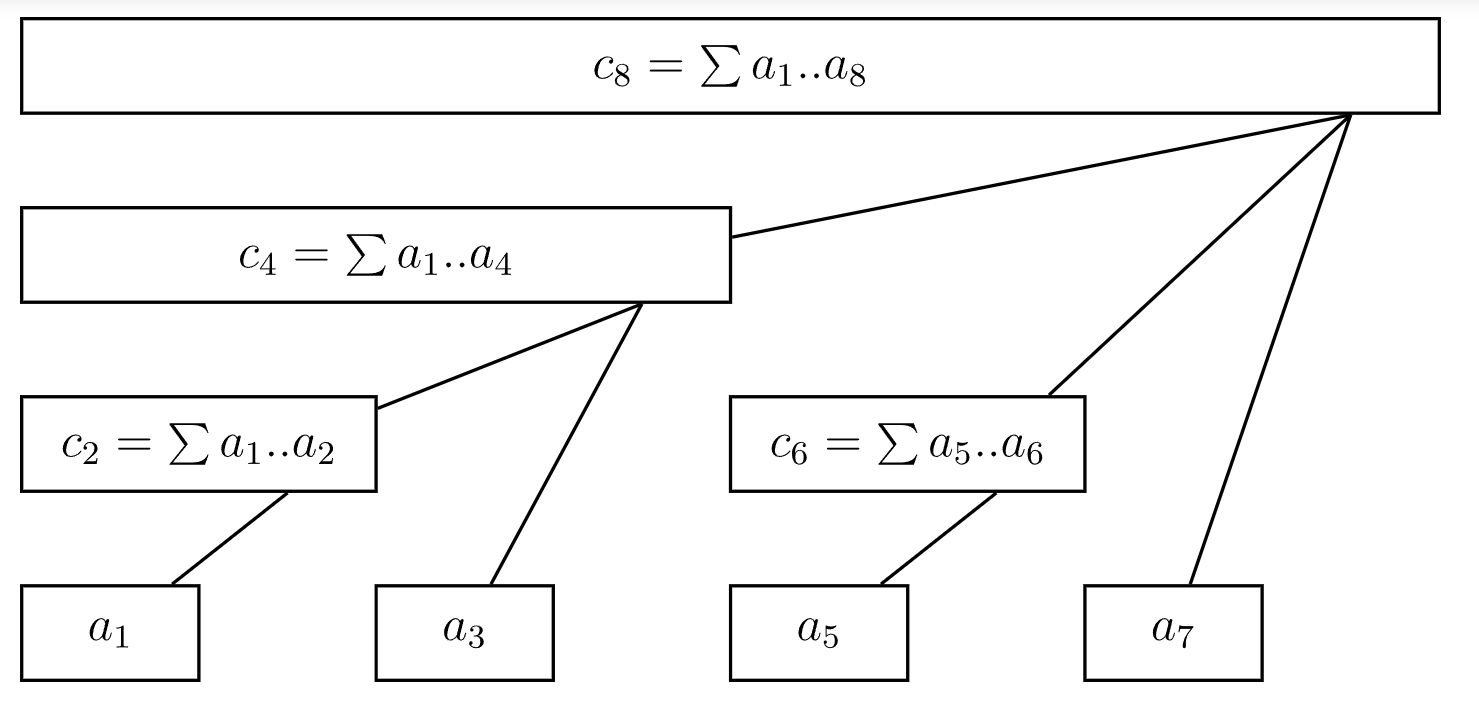
\includegraphics[width=0.7\textwidth,center]{../photo/fenwick}
\subsubsection{单点修改}
\begin{lstlisting}[language=c++]
void update(int num,int x)
{
    for(int i=num;i<=n;i+=lowbit(i)) tre[i]+=x;
}
ll query(int num)
{
    ll sum=0;
    for(int i=num;i>0;i-=lowbit(i)) sum+=tre[i];
    return sum;
}
\end{lstlisting}
\subsubsection{区间修改}
维护序列$a$的差分数组$b$,此时我们对$a$的一个前缀$r$求和,即$\sum_{i=1}^{r}a_i$,由差分数组定义得$a_i=\sum_{j=1}^{i}b_j$。
$$
\begin{aligned}
    &\sum_{i=1}^{r}a_i\\
    =&\sum_{i=1}^{r}\sum_{j=1}^{i}b_j\\
    =&\sum_{i=1}^{r}b_i\times(r-i+1)\\
    =&\sum_{i=1}^{r}b_i\times(r+1)-\sum_{i=1}^{r}b_i\times i
\end{aligned}
$$
区间和可以用两个前缀和相减得到,因此只需要用两个树状数组分别维护$\sum b_i$和$\sum i\times b_i$,就能实现区间求和。
\begin{lstlisting}[language=c++,escapeinside=``]
//`tre1表示b的前缀和,tre2表示b*i的前缀和,b表示原数组的差分数组`
void update(int num,int x)
{ 
    for(int i=num;i<=n;i+=lowbit(i)) tre1[i]+=x,tre2[i]+=num*x;
}
void update(int l,int r,int x)
{
    update(l,x);update(r+1,-x);
}
ll query(ll tre[],int x)
{
    ll sum=0;
    for(int i=x;i>0;i-=lowbit(i)) sum+=tre[i];
    return sum;
}
ll query(int x)
{
    return query(tre1,x)*(x+1)-query(tre2,x);
}
\end{lstlisting}
\subsubsection{查询第$k$小/大元素}
\indent在此处只讨论第$k$小,第$k$大问题可以通过简单计算转化为第$k$小问题。\\
\indent找到最大的$x$满足$\sum_{i=1}^x a_i<k$,那么$x+1$就是我们的答案。在树状数组中,节点是根据$2$的幂划分的,每次可以扩大$2$的幂的长度。令$sum$表示当前的$x$所代表的前缀和,有如下算法找到最大的:
\begin{enumerate}
    \item 求出$depth=\left\lfloor\log_2n\right\rfloor$
    \item 计算$t=\displaystyle\sum_{i=x+1}^{x+2^{depth}} a_i$
    \item 如果$sum+t<k$,则此时扩展成功,将$2^{depth}$累加到$x$上;否则扩展失败,对$x$不进行操作
    \item 将$depth$减$1$,回到步骤$2$,直至$depth$为$0$
\end{enumerate}
\begin{lstlisting}[language=c++,escapeinside=``]
// 权值树状数组查询第k小
int kth(int k) 
{
    int cnt=0,ret=0;
    for(int i=log2(n);~i;--i) //`i与上文depth含义相同`
    {      
        ret+=1<<i; //尝试扩展
        if(ret>=n||cnt+tre[ret]>=k) //`如果扩展失败`
            ret-=1<<i;
        else cnt+=tre[ret]; //`扩展成功后,要更新之前求和的值`
    }
    return ret+1;
}
\end{lstlisting}
\section{线段树}
\subsection{单点修改}
\begin{lstlisting}[language=c++]
struct tree
{
    int l,r,sum;
    int mid(){return (l+r)/2;}
}tre[maxn<<2];
void pushup(int num)
{
    tre[num].sum=tre[2*num].sum+tre[2*num+1].sum;
}
void build(int num,int l,int r)
{
    tre[num].l=l,tre[num].r=r;
    if(l==r)
    {
        tre[num].sum=a[l];return;
    }
    int mid=tre[num].mid();
    build(2*num,l,mid);build(2*num+1,mid+1,r);
    pushup(num);
}
int query(int num,int l,int r)
{
    if(tre[num].l==l && tre[num].r==r)
    return tre[num].sum;
    int mid=tre[num].mid();
    if(l>mid) return query(2*num+1,l,r);
    else if(r<=mid) return query(2*num,l,r);
    else return(query(2*num,l,mid)+query(2*num+1,mid+1,r));
}
void add(int num,int n,int k)
{
    if(tre[num].l==tre[num].r) tre[num].sum+=k;return;
    int mid=tre[num].mid();
    if(n<=mid) add(2*num,n,k);
    else add(2*num+1,n,k);
    pushup(num);
}
\end{lstlisting}
\subsection{区间修改}
\begin{lstlisting}[language=c++]
struct tree
{
    ll l,r,sum,lazy;
    ll mid(){return (l+r)/2;}
}tre[4*maxn];
void build(ll num,ll l,ll r)
{
    tre[num].l=l;tre[num].r=r;
    tre[num].lazy=0;
    if(l==r)
    {
        tre[num].sum=a[l];
        return;
    }
    ll mid=tre[num].mid();
    build(2*num,l,mid);build(2*num+1,mid+1,r);
    tre[num].sum=tre[2*num].sum+tre[2*num+1].sum;
}
void pushdown(ll num)
{
    tre[2*num].sum+=(tre[2*num].r-tre[2*num].l+1)*tre[num].lazy;
    tre[2*num+1].sum+=(tre[2*num+1].r-tre[2*num+1].l+1)*tre[num].lazy;
    tre[2*num].lazy+=tre[num].lazy;
    tre[2*num+1].lazy+=tre[num].lazy;
    tre[num].lazy=0;
}
ll query(ll num,ll l,ll r)
{
    if(tre[num].l==l && tre[num].r==r) return tre[num].sum;
    pushdown(num);
    ll mid=tre[num].mid();
    if(l>mid) return query(2*num+1,l,r);
    else if(r<=mid) return query(2*num,l,r);
    else return query(2*num,l,mid)+query(2*num+1,mid+1,r);
}
void update(ll num,ll l,ll r,ll k)
{
    if(tre[num].l==l && tre[num].r==r)
    {
        tre[num].sum+=(tre[num].r-tre[num].l+1)*k;
        tre[num].lazy+=k;
        return;
    }
    pushdown(num);
    ll mid=tre[num].mid();
    if(l>mid) update(2*num+1,l,r,k);
    else if(r<=mid) update(2*num,l,r,k);
    else
    {
        update(2*num,l,mid,k);update(2*num+1,mid+1,r,k);
    }
    tre[num].sum=tre[2*num].sum+tre[2*num+1].sum;
}
\end{lstlisting}
\section{势能线段树}
\begin{lstlisting}[language=c++,title=区间进行lowbit操作]
struct tree
{
    ll l,r,sum,lazy,flag;
    ll mid(){return (l+r)/2;}
}tre[4*maxn];
int check(int num)
{
    int cnt=0;
    for(int i=32;i>=0;i--) if(tre[num].sum>>i&1) cnt++;
    if(cnt==1) 
    {
        tre[num].sum%=mod;
        return 1;
    }
    return 0;
}
void pushdown(ll num)
{
    int lazy=tre[num].lazy;
    if(lazy==0) return;
    tre[2*num].sum=(tre[2*num].sum*p[lazy])%mod;
    tre[2*num+1].sum=(tre[2*num+1].sum*p[lazy])%mod;
    tre[2*num].lazy+=tre[num].lazy;
    tre[2*num+1].lazy+=tre[num].lazy;
    tre[num].lazy=0;
}
void pushup(int num)
{
    tre[num].sum=(tre[2*num].sum+tre[2*num+1].sum)%mod;
    tre[num].flag=tre[2*num].flag&tre[2*num+1].flag;
}
void build(ll num,ll l,ll r)
{
    tre[num].l=l;tre[num].r=r;
    tre[num].lazy=0;tre[num].sum=0;tre[num].flag=0;
    if(l==r)
    {
        tre[num].sum=a[l];tre[num].flag=check(num);
        return;
    }
    ll mid=tre[num].mid();
    build(2*num,l,mid);build(2*num+1,mid+1,r);
    pushup(num);
}
ll query(ll num,ll l,ll r)
{
    if(tre[num].l==l && tre[num].r==r)
    {
        return tre[num].sum%mod;
    }
    pushdown(num);
    ll mid=tre[num].mid();
    if(l>mid) return query(2*num+1,l,r);
    else if(r<=mid) return query(2*num,l,r);
    else return (query(2*num,l,mid)+query(2*num+1,mid+1,r))%mod;
}
void update(ll num,ll l,ll r)
{
    ll mid=tre[num].mid();
    if(tre[num].l==l && tre[num].r==r)
    {
        if(tre[num].flag)
        {
            tre[num].sum=(tre[num].sum*2)%mod;tre[num].lazy++;
        }
        else
        {
            if(l==r)
            {
                tre[num].sum=lowbit(tre[num].sum)+tre[num].sum;
                tre[num].flag=check(num);
            }
            else
            {
                update(2*num,l,mid);update(2*num+1,mid+1,r);
                pushup(num);
            }

        }
        return;
    }
    pushdown(num);
    if(l>mid) update(2*num+1,l,r);
    else if(r<=mid) update(2*num,l,r);
    else
    {
        update(2*num,l,mid);update(2*num+1,mid+1,r);
    }
    pushup(num);
}
\end{lstlisting}
\section{主席树}
\subsubsection{区间第$k$大}
\begin{lstlisting}[language=c++]
int build(int l,int r)
{
    int pos=++cnt;
    lch[pos]=0,rch[pos]=0,sum[pos]=0;
    if(l<r)
    {
        int mid=l+r>>1;
        lch[pos]=build(l,mid);
        rch[pos]=build(mid+1,r);
    }
    return pos;
}
int update(int pre,int l,int r,ll x)
{
    int pos=++cnt;
    lch[pos]=lch[pre],rch[pos]=rch[pre],sum[pos]=sum[pre];
    if(l<r)
    {
        int mid=l+r>>1;
        if(x<=mid) lch[pos]=update(lch[pre],l,mid,x);
        else rch[pos]=update(rch[pre],mid+1,r,x);
        sum[pos]=sum[lch[pos]]+sum[rch[pos]];
    }
    else sum[pos]++;
    return pos;
}
int query(int x,int y,int l,int r,int k)
{
    if(l==r) return l;
    int mid=l+r>>1;
    int nn=sum[lch[y]]-sum[lch[x]];
    if(nn<k) return query(rch[x],rch[y],mid+1,r,k-nn);
    else return query(lch[x],lch[y],l,mid,k);
}
\end{lstlisting}
\section{树上差分}
\subsection{点差分}
$$
\begin{aligned}
    &d_s \leftarrow d_s+1\\
    &d_{lca} \leftarrow d_{lca}-1\\
    &d_t \leftarrow d_t+1 \\
    &d_{f(lca)} \leftarrow d_{f(lca)}-1
\end{aligned}
$$
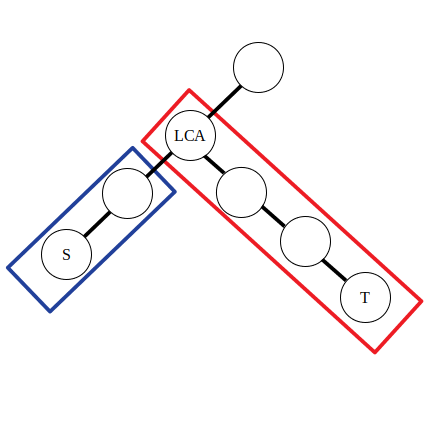
\includegraphics[width=0.4\textwidth,center]{../photo/prefix_sum1.png}
\subsection{边差分}
$$
\begin{aligned}
    &d_s \leftarrow d_s+1\\
    &d_t \leftarrow d_t+1 \\
    &d_{lca} \leftarrow d_{lca}-2\\
\end{aligned}
$$
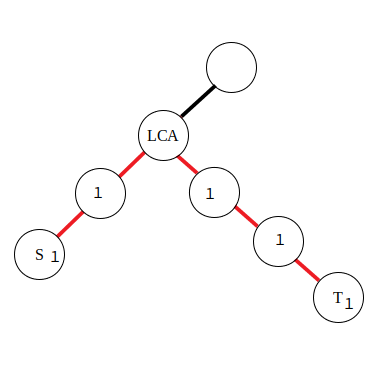
\includegraphics[width=0.4\textwidth,center]{../photo/prefix_sum2.png}
\section{树链剖分}
\subsubsection{重链剖分}
\begin{lstlisting}[language=c++]
void dfs1(int u,int fa)
{
    sz[u]=1;big[u]=-1;dep[u]=dep[fa]+1;par[u]=fa;
    for(auto nex:v[u])
    {
        if(nex==fa) continue;
        dfs1(nex,u);sz[u]+=sz[nex];
        if(big[u]==-1||sz[big[u]]<sz[nex]) big[u]=nex;
    }
}
void dfs2(int u,int fa,int t)
{
    top[u]=t;dfn[u]=++tim;rk[tim]=u;
    if(big[u]==-1) return;
    dfs2(big[u],u,t);
    for(auto nex:v[u])
    {
        if(nex==fa||nex==big[u]) continue;
        dfs2(nex,u,nex);
    }
}
struct SegTree
{
    struct tree
    {
        int l,r;ll sum;
        int mid(){return l+r>>1;}
    }tre[maxn<<2];
    void pushup(int num)
    {
        tre[num].sum=tre[2*num].sum+tre[2*num+1].sum;
    }
    void build(int num,int l,int r)
    {
        tre[num].l=l;tre[num].r=r;
        if(l==r)
        {
            tre[num].sum=a[rk[l]];return;
        }
        int mid=tre[num].mid();
        build(2*num,l,mid);build(2*num+1,mid+1,r);
        pushup(num);
    }
    ll query_sum(int num,int l,int r)
    {
        if(tre[num].l==l&&tre[num].r==r)
        {
            return tre[num].sum;
        }
        int mid=tre[num].mid();
        if(l>mid) return query_sum(2*num+1,l,r);
        else if(r<=mid) return query_sum(2*num,l,r);
        else return query_sum(2*num,l,mid)+query_sum(2*num+1,mid+1,r);
    }
    void update(int num,int pos,int x)
    {
        if(tre[num].l==tre[num].r)
        {
            tre[num].sum=x;return;
        }
        int mid=tre[num].mid();
        if(pos<=mid) update(2*num,pos,x);
        else update(2*num+1,pos,x);
        pushup(num);
    }
}st;
ll query_sum(int x,int y)
{
    ll res=0,fx=top[x],fy=top[y];
    while(fx!=fy)
    {
        if(dep[fx]>=dep[fy]) res+=st.query_sum(1,dfn[fx],dfn[x]),x=par[fx];
        else res+=st.query_sum(1,dfn[fy],dfn[y]),y=par[fy];
        fx=top[x],fy=top[y];
    }
    if(dfn[x]<dfn[y]) res+=st.query_sum(1,dfn[x],dfn[y]);
    else res+=st.query_sum(1,dfn[y],dfn[x]);
    return res;
}
\end{lstlisting}
\section{莫队}
\begin{lstlisting}[language=c++,title=区间不同种类元素个数]
#include<bits/stdc++.h> 
using namespace std;
int n,m,a[50005],vis[1000005],len;
struct node{int l,r,id;}q[200005];
int ans[200005],res=0;
bool cmp(node a,node b)
{
	int al=a.l/len,bl=b.l/len;
	if(al!=bl) return al<bl;
	return a.r<b.r;
}
void add(int num)
{
	vis[a[num]]++;
	if(vis[a[num]]==1) res++;
}
void del(int num)
{
	vis[a[num]]--;
	if(vis[a[num]]==0) res--;
} 
int main()
{
	scanf("%d",&n);len=sqrt(n);
	for(int i=1;i<=n;i++) scanf("%d",&a[i]);
	scanf("%d",&m);
	for(int i=1;i<=m;i++)
	{
		scanf("%d%d",&q[i].l,&q[i].r);q[i].id=i;
	}
	sort(q+1,q+1+m,cmp);
	int l=1,r=0;
	for(int i=1;i<=m;i++)
	{
		int id=q[i].id,ll=q[i].l,rr=q[i].r;
		while(r<rr) add(++r);
		while(r>rr) del(r--);
		while(l<ll) del(l++);
		while(l>ll) add(--l);
		ans[id]=res;
	}
	for(int i=1;i<=m;i++) printf("%d\n",ans[i]);
}
\end{lstlisting}
\ifx\allfiles\undefined
\end{document}
\fi

